\subsection{Fase di progettazione architetturale}

\subsubsection{Progettazione della technology baseline}

I dati riportati di seguito si riferiscono al periodo che va dal 25-01-2021 al 08-02-2021.

\begin{minipage}[b]{0.65\linewidth}
\begin{small}
{
\setlength\arrayrulewidth{1pt}
\begin{longtable}{ c | c c c c c c | c} 
 \rowcolor{coloreRosso}
 \color{white}{\textbf{Nominativo}} &
 \color{white}{\textbf{RE}} &
 \color{white}{\textbf{AM}} &
 \color{white}{\textbf{AN}} &
 \color{white}{\textbf{PT}} &
 \color{white}{\textbf{PR}} &
 \color{white}{\textbf{VE}} &
 \color{white}{\textbf{Tot.}} \\
 	
 \BM{} & - & 2 & 2 & 4 & - & 4 & 12 \\ 
 \PA{} & 4 & - & 5 & 3 & - & - & 12 \\ 
 \RA{} & - & - & 5 & - & 4 & 5 & 10 \\ 
 \SH{} & - & - & 2 & 5 & - & 3 & 14 \\ 
 \SG{} & - & 3 & - & 4 & - & 5 & 12 \\ 
 \SP{} & - & 3 & - & 5 & - & 6 & 14 \\ 
 \ZM{} & - & - & 5 & 3 & - & 4 & 12 \\
 
 	\rowcolor{coloreRosso}
 	\color{white}{\textbf{Totale ore ruolo}} &
 	\color{white}{\textbf{4}} &
 	\color{white}{\textbf{8}} &
 	\color{white}{\textbf{19}} &
 	\color{white}{\textbf{24}} &
 	\color{white}{\textbf{4}} &
 	\color{white}{\textbf{27}} &
 	\color{white}{\textbf{86}} \\
	\rowcolor{white}
	\captionsetup{width=1\textwidth}
 	\caption{Distribuzione delle ore nella progettazione della TB}
\end{longtable}
}
\end{small}
\end{minipage}
\begin{minipage}[b]{.3\linewidth}
\begin{small}
{
\setlength\arrayrulewidth{1pt}
\begin{longtable}{ c | c | c} 
 	\rowcolor{coloreRosso}
 	\color{white}{\textbf{Ruolo}} &
 	\color{white}{\textbf{Ore}} &
 	\color{white}{\textbf{Costo €}} \\
 	
 	Responsabile & 4 & 120\\
 	Amministratore & 8 & 160\\
 	Analista & 19 & 475\\
 	Progettista & 24 & 528\\
 	Programmatore & 4 & 60\\
 	Verificatore & 27 & 405\\
 	
 	\rowcolor{coloreRosso}
 	\color{white}{\textbf{Totale}} &
 	\color{white}{\textbf{86}} &
 	\color{white}{\textbf{1748}}\\
 	\rowcolor{white}
 	\caption{Costi per ruolo nella progettazione della TB}
\end{longtable}
}
\end{small}
\end{minipage}

\begin{figure}[!htb]   
    \centering
    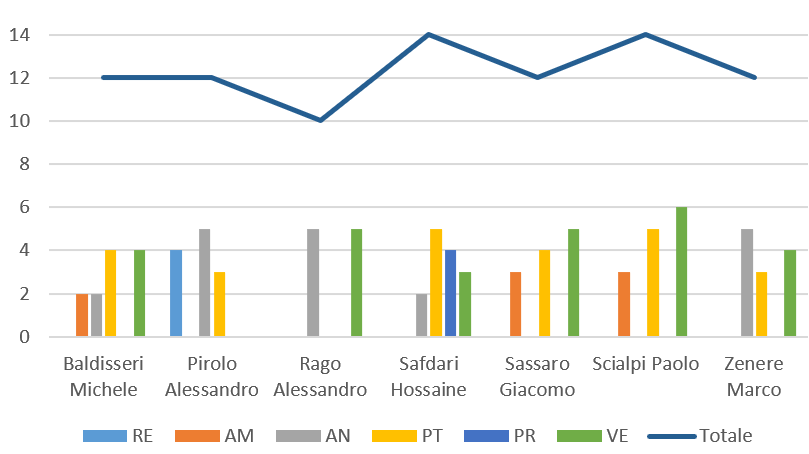
\includegraphics[width=0.9\textwidth]{Images/per1}
	\caption{Ripartizione oraria per ciascun membro nella progettazione della TB}
\end{figure}

\subsubsection{Progettazione e codifica del Proof of Concept}
\paragraph{Incremento I}\mbox{} \\
I dati riportati di seguito si riferiscono al periodo che va dall' 08-02-2021 al 18-02-2021.

\begin{minipage}[b]{0.65\linewidth}
\begin{small}
{
\setlength\arrayrulewidth{1pt}
\begin{longtable}{ c | c c c c c c | c} 
 \rowcolor{coloreRosso}
 \color{white}{\textbf{Nominativo}} &
 \color{white}{\textbf{RE}} &
 \color{white}{\textbf{AM}} &
 \color{white}{\textbf{AN}} &
 \color{white}{\textbf{PT}} &
 \color{white}{\textbf{PR}} &
 \color{white}{\textbf{VE}} &
 \color{white}{\textbf{Tot.}} \\
 	
 \BM{} & - & 4 & 3 & 5 & - & - & 12 \\ 
 \PA{} & 2 & - & - & - & 5 & 4 & 11 \\ 
 \RA{} & - & - & 6 & 2 & 2 & 2 & 12 \\ 
 \SH{} & - & - & 3 & 2 & 1 & 3 & 9 \\ 
 \SG{} & - & 5 & 3 & 5 & - & - & 13 \\ 
 \SP{} & - & 3 & - & 3 & 6 & - & 12 \\ 
 \ZM{} & - & - & 5 & 7 & - & - & 12 \\
 
 	\rowcolor{coloreRosso}
 	\color{white}{\textbf{Totale ore ruolo}} &
 	\color{white}{\textbf{2}} &
 	\color{white}{\textbf{12}} &
 	\color{white}{\textbf{20}} &
 	\color{white}{\textbf{24}} &
 	\color{white}{\textbf{14}} &
 	\color{white}{\textbf{9}} &
 	\color{white}{\textbf{81}} \\
	\rowcolor{white}
	\captionsetup{width=.9\textwidth}
 	\caption{Distribuzione delle ore nell'incremento I}
\end{longtable}
}
\end{small}
\end{minipage}
\begin{minipage}[b]{.3\linewidth}
\begin{small}
{
\setlength\arrayrulewidth{1pt}
\begin{longtable}{ c | c | c} 
 	\rowcolor{coloreRosso}
 	\color{white}{\textbf{Ruolo}} &
 	\color{white}{\textbf{Ore}} &
 	\color{white}{\textbf{Costo €}} \\
 	
 	Responsabile & 2 & 60\\
 	Amministratore & 12 & 240\\
 	Analista & 20 & 500\\
 	Progettista & 24 & 528\\
 	Programmatore & 14 & 210\\
 	Verificatore & 9 & 135\\
 	
 	\rowcolor{coloreRosso}
 	\color{white}{\textbf{Totale}} &
 	\color{white}{\textbf{81}} &
 	\color{white}{\textbf{1673}}\\
 	\rowcolor{white}
 	\caption{Costi per ruolo nell'incremento I}
\end{longtable}
}
\end{small}
\end{minipage}

\begin{figure}[!htb]   
    \centering
    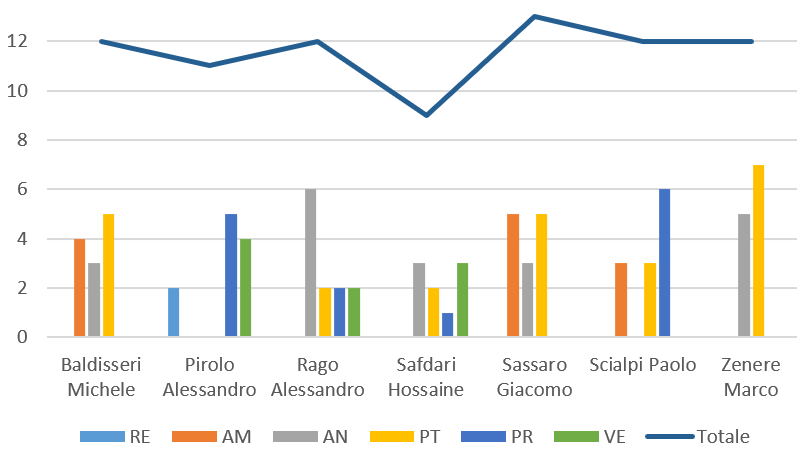
\includegraphics[width=0.9\textwidth]{Images/per2}
	\caption{Ripartizione oraria per ciascun membro nell'incremento I}
\end{figure}

\paragraph{Incremento II}\mbox{} \\
I dati riportati di seguito si riferiscono al periodo che va dal 18-02-2021 al 01-03-2021.

\begin{minipage}[b]{0.65\linewidth}
\begin{small}
{
\setlength\arrayrulewidth{1pt}
\begin{longtable}{ c | c c c c c c | c} 
 \rowcolor{coloreRosso}
 \color{white}{\textbf{Nominativo}} &
 \color{white}{\textbf{RE}} &
 \color{white}{\textbf{AM}} &
 \color{white}{\textbf{AN}} &
 \color{white}{\textbf{PT}} &
 \color{white}{\textbf{PR}} &
 \color{white}{\textbf{VE}} &
 \color{white}{\textbf{Tot.}} \\
 	
 \BM{} & - & 3 & 2 & - & 3 & - & 8 \\ 
 \PA{} & - & - & - & 4 & - & 5 & 9 \\ 
 \RA{} & - & - & - & 6 & 4 & - & 10 \\ 
 \SH{} & - & - & - & 2 & 3 & 4 & 9 \\ 
 \SG{} & - & 1 & 2 & - & 4 & - & 7 \\ 
 \SP{} & - & 6 & - & - & - & - & 6 \\ 
 \ZM{} & 6 & - & - & - & 2 & - & 8 \\
 
 	\rowcolor{coloreRosso}
 	\color{white}{\textbf{Totale ore ruolo}} &
 	\color{white}{\textbf{6}} &
 	\color{white}{\textbf{10}} &
 	\color{white}{\textbf{4}} &
 	\color{white}{\textbf{12}} &
 	\color{white}{\textbf{16}} &
 	\color{white}{\textbf{9}} &
 	\color{white}{\textbf{57}} \\
	\rowcolor{white}
	\captionsetup{width=.9\textwidth}
 	\caption{Distribuzione delle ore nell'incremento II}
\end{longtable}
}
\end{small}
\end{minipage}
\begin{minipage}[b]{.3\linewidth}
\begin{small}
{
\setlength\arrayrulewidth{1pt}
\begin{longtable}{ c | c | c} 
 	\rowcolor{coloreRosso}
 	\color{white}{\textbf{Ruolo}} &
 	\color{white}{\textbf{Ore}} &
 	\color{white}{\textbf{Costo €}} \\
 	
 	Responsabile & 6 & 180\\
 	Amministratore & 10 & 200\\
 	Analista & 4 & 100\\
 	Progettista & 12 & 264\\
 	Programmatore & 16 & 240\\
 	Verificatore & 9 & 135\\
 	
 	\rowcolor{coloreRosso}
 	\color{white}{\textbf{Totale}} &
 	\color{white}{\textbf{57}} &
 	\color{white}{\textbf{1119}}\\
 	\rowcolor{white}
 	\caption{Costi per ruolo nell'incremento II}
\end{longtable}
}
\end{small}
\end{minipage}

\begin{figure}[!htb]   
    \centering
    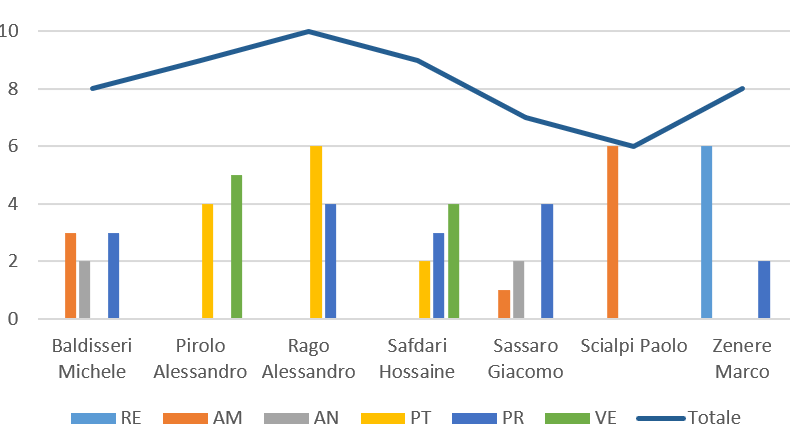
\includegraphics[width=0.9\textwidth]{Images/per3}
	\caption{Ripartizione oraria per ciascun membro nell'incremento II}
\end{figure}

\subsubsection{Riepilogo}

\begin{minipage}[b]{0.65\linewidth}
\begin{small}
{
\setlength\arrayrulewidth{1pt}
\begin{longtable}{ c | c c c c c c | c} 
 \rowcolor{coloreRosso}
 \color{white}{\textbf{Nominativo}} &
 \color{white}{\textbf{RE}} &
 \color{white}{\textbf{AM}} &
 \color{white}{\textbf{AN}} &
 \color{white}{\textbf{PT}} &
 \color{white}{\textbf{PR}} &
 \color{white}{\textbf{VE}} &
 \color{white}{\textbf{Tot.}} \\
 	
 \BM{} & - & 9 & 7 & 9 & 3 & 4 & 32 \\ 
 \SG{} & - & 9 & 5 & 9 & 4 & 5 & 32 \\ 
 \SH{} & - & - & 5 & 9 & 8 & 10 & 32 \\ 
 \PA{} & 6 & - & 5 & 7 & 5 & 9 & 32 \\ 
 \SP{} & - & 12 & - & 8 & 6 & 6 & 32 \\ 
 \RA{} & - & - & 11 & 8 & 6 & 7 & 32 \\ 
 \ZM{} & 6 & - & 10 & 10 & 2 & 4 & 32 \\
 
 	\rowcolor{coloreRosso}
 	\color{white}{\textbf{Totale ore ruolo}} &
 	\color{white}{\textbf{12}} &
 	\color{white}{\textbf{30}} &
 	\color{white}{\textbf{43}} &
 	\color{white}{\textbf{60}} &
 	\color{white}{\textbf{34}} &
 	\color{white}{\textbf{45}} &
 	\color{white}{\textbf{224}} \\
	\rowcolor{white}
	\captionsetup{width=.9\textwidth}
 	\caption{Distribuzione delle ore nella fase di progettazione architetturale}
\end{longtable}
}
\end{small}
\end{minipage}
\begin{minipage}[b]{.3\linewidth}
\begin{small}
{
\setlength\arrayrulewidth{1pt}
\begin{longtable}{ c | c | c} 
 	\rowcolor{coloreRosso}
 	\color{white}{\textbf{Ruolo}} &
 	\color{white}{\textbf{Ore}} &
 	\color{white}{\textbf{Costo €}} \\
 	
 	Responsabile & 12 & 360\\
 	Amministratore & 30 & 600\\
 	Analista & 43 & 1075\\
 	Progettista & 60 & 1320\\
 	Programmatore & 34 & 510\\
 	Verificatore & 45 & 675\\
 	
 	\rowcolor{coloreRosso}
 	\color{white}{\textbf{Totale}} &
 	\color{white}{\textbf{224}} &
 	\color{white}{\textbf{4540}}\\
 	\rowcolor{white}
 	\caption{Costi per ruolo nella fase di progettazione architetturale}
\end{longtable}
}
\end{small}
\end{minipage}

I seguenti grafici riassumo i dati ottenuti.

\begin{figure}[!htb]
   \begin{minipage}{0.6\textwidth}
     \centering
     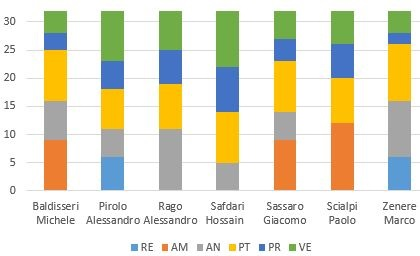
\includegraphics{Images/PO-Progettazione}
     \caption{Ripartizione oraria per ciascun membro nella fase di progettazione architetturale}
   \end{minipage}\hspace{0.1\textwidth}
   \begin{minipage}{0.3\textwidth}
     \centering
     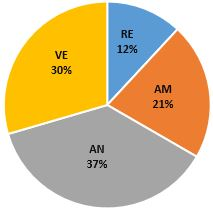
\includegraphics[width=.9\textwidth]{Images/PE-Analisi}
     \captionsetup{width=1.1\textwidth}
     \caption{Ripartizione ore totali nella fase di progettazione architetturale}
   \end{minipage}
\end{figure}